\documentclass[12pt,a4paper]{report}
\usepackage[utf8]{inputenc}
\usepackage{graphicx}
\usepackage{amsmath}
\usepackage{geometry}
\geometry{a4paper, margin=1in}
\usepackage{times}
\usepackage{titlesec}
\usepackage{caption}
\usepackage{float}
\usepackage{setspace}
\usepackage{booktabs}

\titleformat{\chapter}[display]{\normalfont\huge\bfseries}{\chaptertitlename\ \thechapter}{20pt}{\Huge}
\titlespacing*{\chapter}{0pt}{-50pt}{40pt}

\onehalfspacing

\begin{document}

% --- Cover Page ---
\begin{titlepage}
\begin{center}
{\fontsize{28}{34}\selectfont\bfseries Comprehensive Analysis of Field Oriented Control (FOC) for a 3-Phase Induction Motor\par}
\vspace{1.5cm}
{\fontsize{14}{17}\selectfont Project Report Submitted in partial fulfilment of the requirements for the degree of Bachelor of Technology from Maulana Abul Kalam Azad University of Technology, West Bengal (formerly known as West Bengal University of Technology)\par}
\vspace{1.5cm}
{\Large \bfseries By\par}
\vspace{0.5cm}
{\fontsize{18}{22}\selectfont\bfseries
SURJA MONDAL (Roll No. 34901622011)\\
JOYDIP KARMAKAR (Roll No. 34901622014)\\
ANGSU PRIYA ROY (Roll No. 34901622020)\\
HIRAK SINHA (Roll No. 34901622042)\\
KESHAB SARKAR (Roll No. 34901622044)\par}
\vspace{1.5cm}
{\fontsize{16}{19}\selectfont Under the Guidance of\par}
\vspace{0.5cm}
{\fontsize{16}{19}\selectfont Prof. Deepjyoti Santra\par}
\vfill
{\Large Department of Electrical Engineering\par}
{\Large Cooch Behar Government Engineering College\par}
{\Large Cooch Behar, West Bengal\par}
{\Large 2026\par}
\end{center}
\end{titlepage}

% --- Certificate of Recommendation ---
\newpage
\begin{center}
{\Large \bfseries Certificate of Recommendation\par}
\end{center}
\vspace{1cm}
It is hereby recommended to consider the project report entitled \textbf{``Comprehensive Analysis of Field Oriented Control (FOC) for a 3-Phase Induction Motor''} submitted by SURJA MONDAL (Roll No. 34901622011), JOYDIP KARMAKAR (Roll No. 34901622014), ANGSU PRIYA ROY (Roll No. 34901622020), HIRAK SINHA (Roll No. 34901622042), and KESHAB SARKAR (Roll No. 34901622044) for partial fulfillment of the requirements for the award of the degree of Bachelor of Technology in Electrical Engineering from Maulana Abul Kalam Azad University of Technology (formerly known as West Bengal University of Technology).
\vspace{3cm}

\noindent
\begin{tabular}{@{}p{8cm}p{8cm}@{}}
------------------------------ & ------------------------------- \\
Prof. Deepjyoti Santra & Prof. Atanu Maji \\
Project Guide & (Head of Electrical Engg. Department)
\end{tabular}

% --- Certificate of Approval ---
\newpage
\begin{center}
{\Large \bfseries Certificate of Approval\par}
\end{center}
\vspace{1cm}
It is hereby approved that the project report entitled \textbf{``Comprehensive Analysis of Field Oriented Control (FOC) for a 3-Phase Induction Motor''} submitted by SURJA MONDAL (Roll No. 34901622011), JOYDIP KARMAKAR (Roll No. 34901622014), ANGSU PRIYA ROY (Roll No. 34901622020), HIRAK SINHA (Roll No. 34901622042), and KESHAB SARKAR (Roll No. 34901622044) for partial fulfilment of the requirements for the award of the degree of Bachelor of Technology in Electrical Engineering from Maulana Abul Kalam Azad University of Technology (formerly known as West Bengal University of Technology).
\vspace{3cm}

\noindent \textbf{Board of Examiners}
\vspace{1.5cm}

\noindent 1. --------------------------- \\
\vspace{1cm}

\noindent 2. --------------------------- \\
\vspace{1cm}

\noindent 3. ---------------------------

% --- Acknowledgement ---
\newpage
\begin{center}
{\Large \bfseries Acknowledgement\par}
\end{center}
\vspace{1cm}
We would like to express our profound gratitude to our project guide, Prof. Deepjyoti Santra, for his valuable guidance, continuous support, and encouragement throughout the course of this project. His deep knowledge and technical insights into electrical drives and vector control have been instrumental in shaping this analysis.

We are also deeply thankful to Prof. Atanu Maji, Head of the Electrical Engineering Department, for providing us with the necessary academic framework, laboratory facilities, and a conducive environment to carry out this work successfully. 

We also extend our heartfelt thanks to the faculty, staff, and administration of Cooch Behar Government Engineering College for their continuous assistance and cooperation.

\vspace{2cm}
\begin{flushright}
SURJA MONDAL (34901622011)\\
JOYDIP KARMAKAR (34901622014)\\
ANGSU PRIYA ROY (34901622020)\\
HIRAK SINHA (34901622042)\\
KESHAB SARKAR (34901622044)
\end{flushright}

% --- TOC, LOF, LOT ---
\newpage
\tableofcontents
\newpage
\listoffigures
\newpage
\listoftables

% --- Abstract ---
\newpage
\begin{center}
{\Large \bfseries Abstract\par}
\end{center}
\vspace{1cm}
This report provides a comprehensive, component-level technical analysis of the Simulink model \texttt{VECTOR\_CONTROL\_FOC\_OF\_IM\_2023.slx}, which implements an Indirect Field Oriented Control (IFOC) architecture for a 50 HP Squirrel-Cage Induction Motor. Intended to bridge complex electromechanical theory with practical digital control implementation, this report systematically deconstructs the frameworks embedded within the simulation. It establishes the plant's equivalent circuit parameters and models the dynamic transient response of the decoupling matrices. 

The analysis explores the critical coordinate transformations (Forward and Reverse Clarke and Park) required to map stationary three-phase variables into a synchronously rotating $d-q$ reference frame. By meticulously evaluating the system's decoupling equations, the report demonstrates how IFOC achieves independent, high-performance regulation of rotor flux and electromagnetic torque, mirroring the dynamics of a separately excited DC machine. Furthermore, the discrete-time closed-loop control strategy is examined, detailing the tuning parameters of the cascaded Proportional-Integral (PI) controllers and slip estimation. Finally, the report dissects the Space Vector Pulse Width Modulation (SVPWM) synthesis used to drive the three-phase inverter, verifying its advantages in optimising DC bus voltage utilisation and minimising total harmonic distortion.

% --- Chapter 1 ---
\chapter{Introduction}
\section{Introduction to Field Oriented Control}
Traditionally, the control of induction machines was dominated by scalar methods, such as constant Volts-per-Hertz ($V/f$) control. While adequate for basic steady-state operations, scalar control governs only the magnitude and frequency of the applied voltage and currents, fundamentally ignoring the spatial orientation of the electromagnetic fields. Consequently, scalar methods suffer from sluggish transient responses, cross-coupling effects, and an inability to independently regulate torque and flux during dynamic state changes.

Field Oriented Control (FOC), also known as Vector Control, represents a revolutionary paradigm shift in AC machine drives, overcoming the limitations of scalar control. The fundamental objective of FOC is to emulate the highly desirable, decoupled control dynamics of a separately excited DC motor. In a traditional DC machine, the field flux and the armature flux are maintained in a strict state of spatial orthogonality (perpendicularity) by the mechanical commutator. This decoupling allows the field current and armature current to be manipulated independently to control magnetic flux and electromagnetic torque.

\begin{figure}[H]
    \centering
    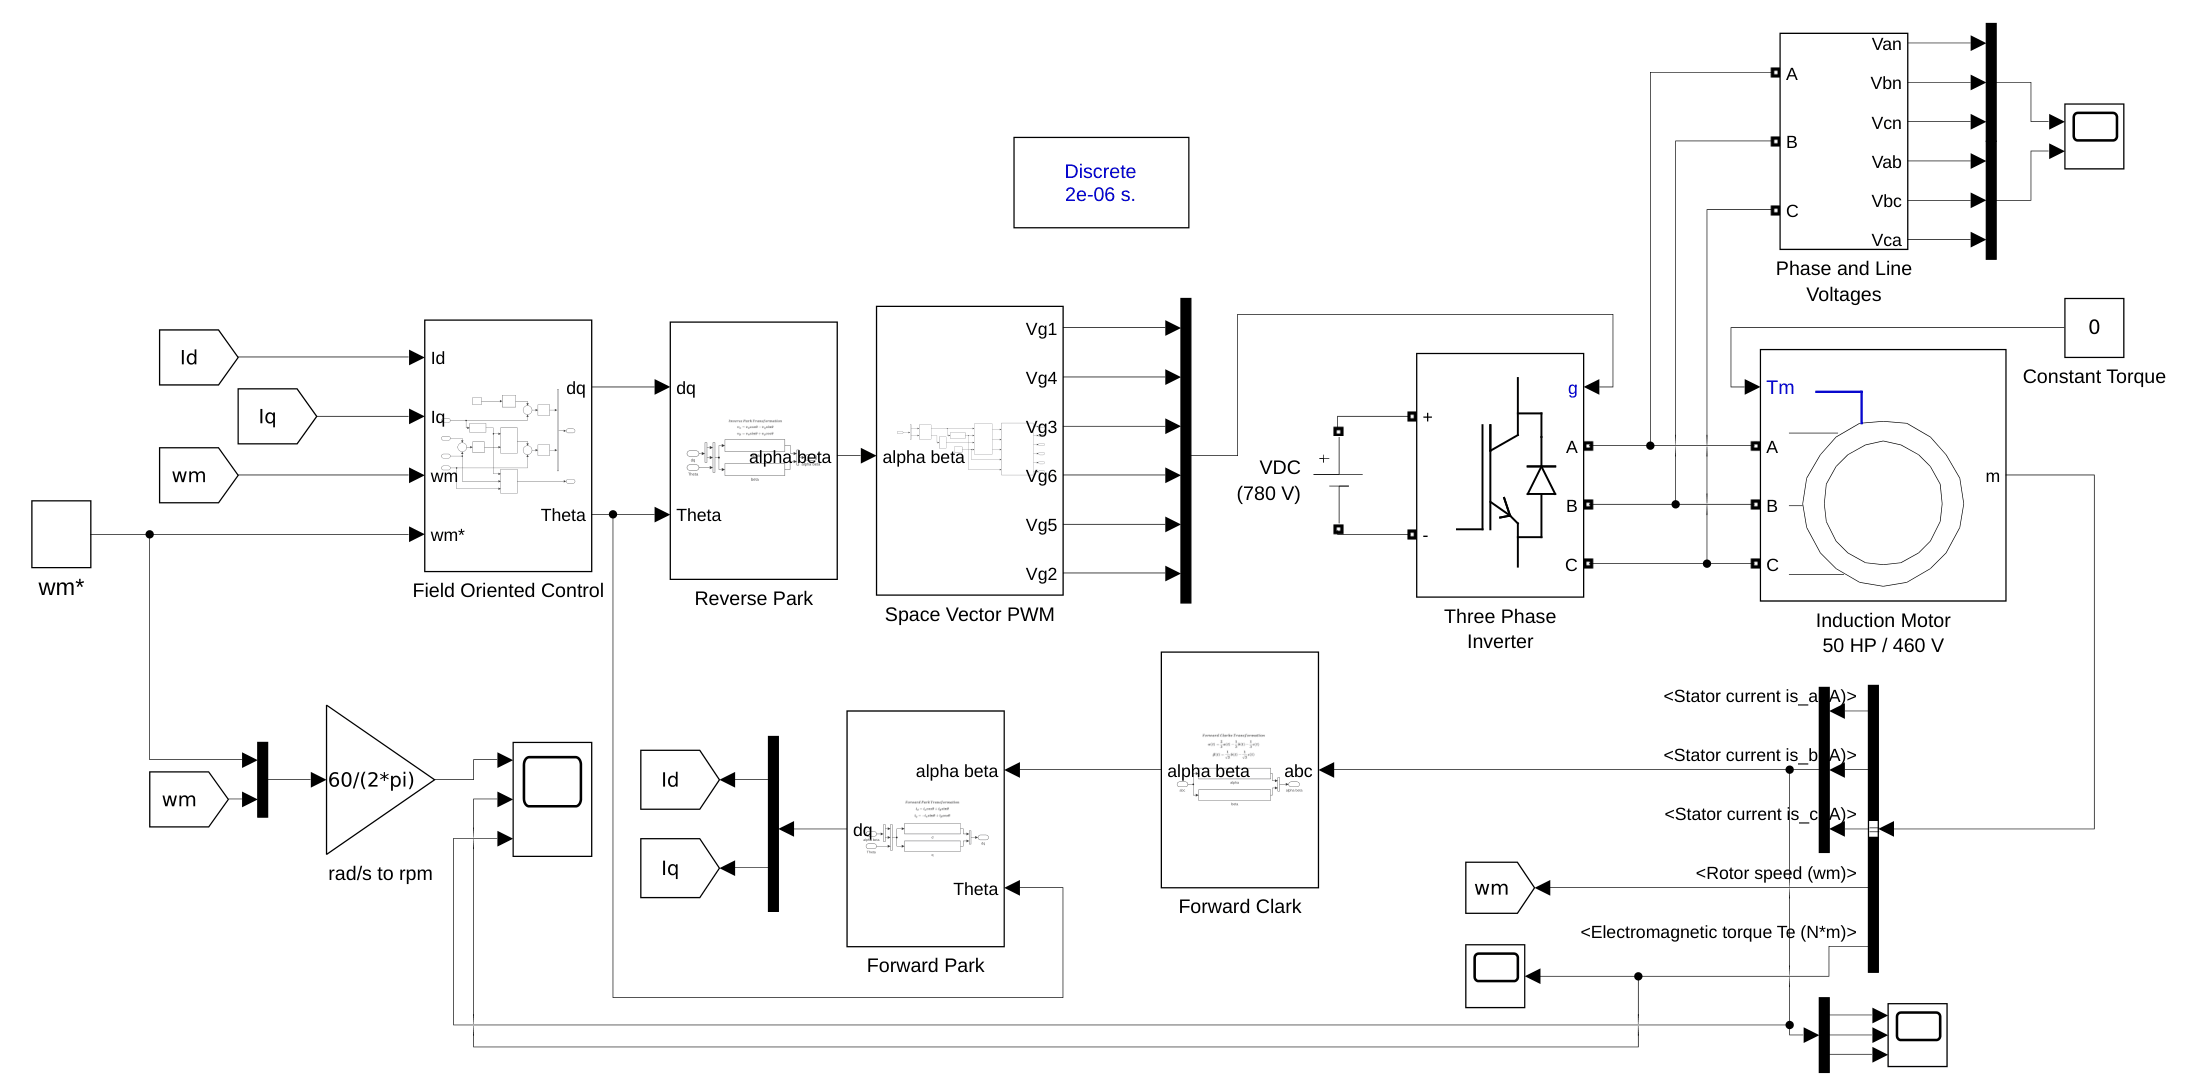
\includegraphics[width=0.95\textwidth]{VECTOR_CONTROL_FOC_OF_IM-01.png}
    \caption{Top-Level Simulink Model Architecture of the FOC for Induction Motor}
    \label{fig:top_level}
\end{figure}

To replicate this orthogonal decoupling in a three-phase AC induction machine, FOC treats the multi-phase stator currents as spatial vectors. Through rigorous mathematical coordinate transformations---the Clarke and Park transforms---the time-varying, three-phase AC variables ($i_{a}, i_{b}, i_{c}$) are projected onto a two-dimensional, synchronously rotating reference frame ($d-q$ axes).

By deliberately aligning the direct-axis ($d$-axis) of this rotating frame with the rotor flux linkage vector, the overall stator current is mathematically decomposed into two entirely independent components:
\begin{itemize}
    \item \textbf{Flux-Producing Component ($i_{ds}$):} The direct-axis stator current is constrained to align perfectly with the rotor flux linkage vector ($\psi_{r}$). It is strictly responsible for establishing and maintaining the internal magnetisation of the machine.
    \item \textbf{Torque-Producing Component ($i_{qs}$):} The quadrature-axis stator current is maintained precisely at a $90^\circ$ electrical angle relative to the rotor flux axis. Because the entirety of the machine's flux is mathematically isolated onto the d-axis ($\psi_{qr}=0$), the torque generation relies exclusively on this component.
\end{itemize}

\section{Torque Calculation and Decoupling}
The developed electromagnetic torque can be expressed via the decoupled equation:
\begin{equation}
T_{e} = \frac{3}{2} \left(\frac{P}{2}\right) \frac{L_{m}}{L_{r}} \psi_{r} i_{qs}
\end{equation}

Based on the parameters defined for the 50 HP motor:
\begin{itemize}
    \item Number of poles, $P = 4$
    \item Magnetizing inductance, $L_{m} = 34.7 \text{ mH} = 0.0347 \text{ H}$
    \item Rotor inductance, $L_{r} = L_{lr} + L_{m} = 0.8 \text{ mH} + 34.7 \text{ mH} = 35.5 \text{ mH} = 0.0355 \text{ H}$
    \item Nominal flux, $\psi_{r} = 0.96 \text{ Wb}$
\end{itemize}

Executing the calculation yields the direct torque constant:
\begin{align}
T_{e} &= \frac{3}{2} \left(\frac{4}{2}\right) \left(\frac{0.0347}{0.0355}\right) (0.96) \cdot i_{qs} \\
T_{e} &= 3 \times (0.9775) \times (0.96) \cdot i_{qs} \\
T_{e} &\approx 2.8152 \cdot i_{qs} \text{ N}\cdot\text{m}
\end{align}

This confirms a direct, linear torque constant of $2.8152 \text{ Nm/A}$ for the q-axis current. Because the rotor flux $\psi_{r}$ is held constant by the independent d-axis control loop, the electromagnetic torque $T_{e}$ becomes directly, linearly, and instantaneously proportional to $i_{qs}$, eliminating cross-coupling dynamics.

\begin{figure}[H]
    \centering
    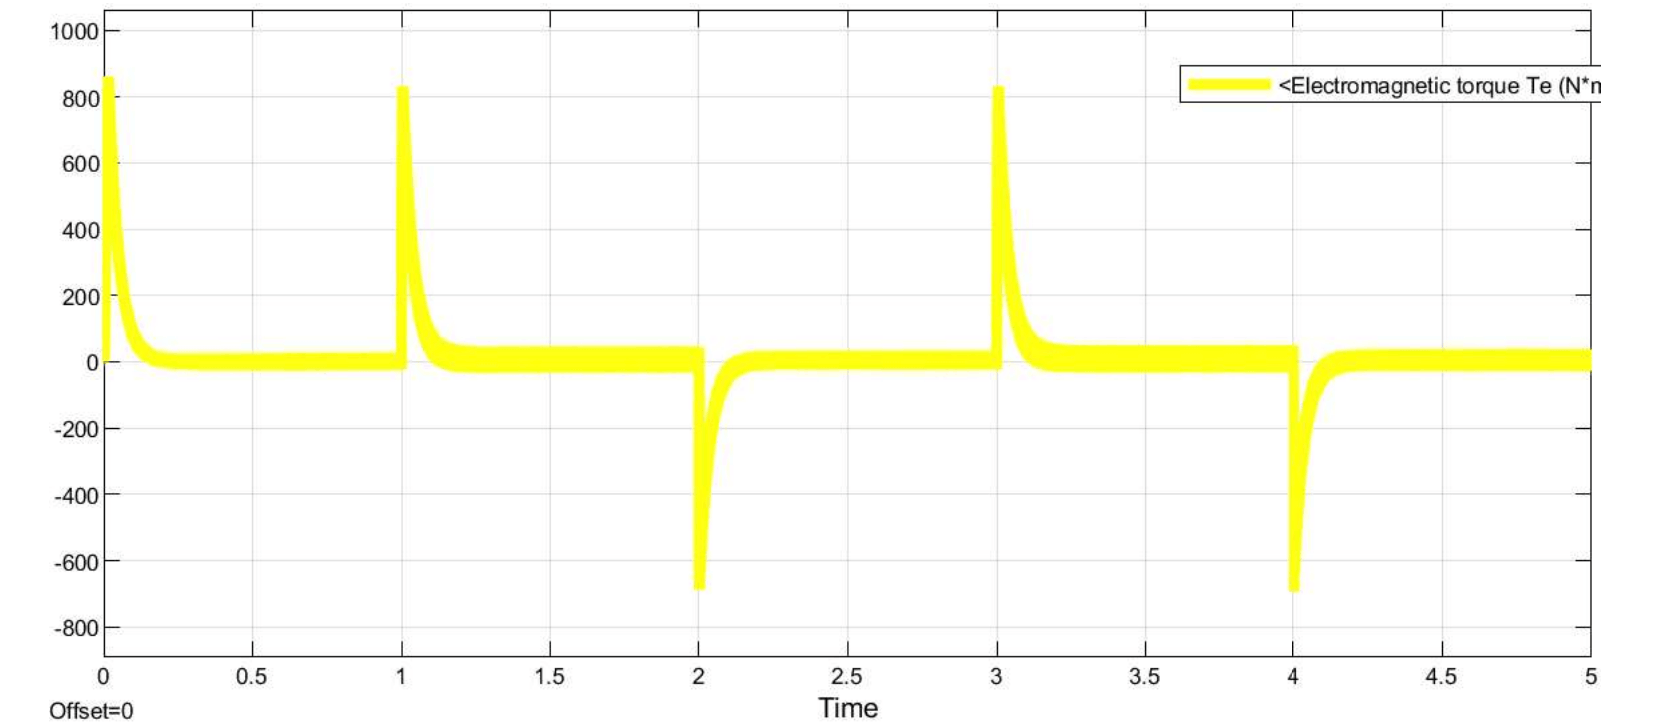
\includegraphics[width=0.9\textwidth]{1.png}
    \caption{Scope Output: Transient and Steady-State Electromechanical Torque ($T_e$) Tracking the Load Demands}
    \label{fig:torque_response}
\end{figure}

% --- Chapter 2 ---
\chapter{Induction Motor Plant Parameters and Dynamic Modelling}
\section{Plant Parameters}
The electromechanical plant governed by this control architecture is a three-phase Squirrel-Cage Induction Motor (SCIM). Because the rotor currents and rotor flux linkages are physically inaccessible and cannot be directly measured, the control strategy relies entirely on an accurate mathematical model of the machine.

\begin{table}[H]
\centering
\caption{Squirrel-Cage Induction Motor Nominal Ratings and Equivalent Circuit Parameters}
\label{tab:motor_params}
\begin{tabular}{llc}
\toprule
\textbf{Symbol} & \textbf{Parameter Description} & \textbf{Value} \\
\midrule
\multicolumn{3}{c}{\textbf{Nominal Ratings}} \\
\midrule
$S$ & Nominal Power & 50 HP (37.3 kW) \\
$V_{s}$ & Stator Line-to-Line Voltage & 460 V \\
$f$ & Nominal Frequency & 50 Hz \\
$P$ & Number of Poles & 4 (2 Pole Pairs) \\
$N_{s}$ & Synchronous Speed & 1500 RPM \\
\midrule
\multicolumn{3}{c}{\textbf{Electrical Parameters (Per Phase)}} \\
\midrule
$R_{s}$ & Stator Resistance & 0.087 $\Omega$ \\
$R_{r}$ & Rotor Resistance (Referred to Stator) & 0.228 $\Omega$ \\
$L_{ls}$ & Stator Leakage Inductance & 0.1 mH \\
$L_{lr}$ & Rotor Leakage Inductance (Referred) & 0.8 mH \\
$L_{m}$ & Magnetizing Inductance & 34.7 mH \\
\midrule
\multicolumn{3}{c}{\textbf{Mechanical Parameters}} \\
\midrule
$J$ & Moment of Inertia & 0.662 kg$\cdot$m$^2$ \\
$F$ & Viscous Friction Coefficient & 0.1 N$\cdot$ms/rad \\
\bottomrule
\end{tabular}
\end{table}

\section{Significance of Electrical Parameters in FOC}
From the raw parameters provided in Table \ref{tab:motor_params}, the lumped self-inductances of the stator ($L_s$) and rotor ($L_r$) are derived as follows:
\begin{align}
L_{s} &= L_{ls} + L_{m} = 0.1 \text{ mH} + 34.7 \text{ mH} = 34.8 \text{ mH} = 0.0348 \text{ H} \\
L_{r} &= L_{lr} + L_{m} = 0.8 \text{ mH} + 34.7 \text{ mH} = 35.5 \text{ mH} = 0.0355 \text{ H}
\end{align}

A critical derived parameter for Indirect FOC is the rotor time constant ($\tau_r$). This value dictates the feedforward slip frequency calculation:
\begin{equation}
\tau_{r} = \frac{L_{r}}{R_{r}} = \frac{0.0355}{0.228} = 0.15570175 \text{ s} \approx 0.1557 \text{ s}
\end{equation}

Furthermore, the machine's total leakage factor ($\sigma$), which dictates the maximum rate of change of stator currents (and thus the necessary bandwidth of the inner PI current controllers), is calculated as:
\begin{align}
\sigma &= 1 - \frac{L_{m}^2}{L_{s}L_{r}} \\
\sigma &= 1 - \frac{(0.0347)^2}{(0.0348 \times 0.0355)} \\
\sigma &= 1 - \frac{0.00120409}{0.0012354} \\
\sigma &= 1 - 0.97465 = 0.02535
\end{align}
This highly coupled magnetic relationship ($\sigma \ll 1$) confirms a well-designed motor but necessitates high-gain, fast-acting current loops to force the stator currents to track the instantaneous FOC references.

\section{Mechanical Dynamics and Speed Loop Tuning}
The mechanical equation of motion that dictates the rotor's dynamic trajectory is governed by:
\begin{equation}
T_{e} - T_{L} = J\frac{d\omega_{m}}{dt} + F\omega_{m}
\end{equation}
Substituting the mechanical parameters of the 50 HP motor ($J=0.662$ and $F=0.1$):
\begin{equation}
T_{e} - T_{L} = 0.662\frac{d\omega_{m}}{dt} + 0.1\cdot\omega_{m}
\end{equation}

Assuming the load torque $T_L = 0$ for the primary plant transfer function analysis, taking the Laplace transform yields:
\begin{equation}
\frac{\omega_{m}(s)}{T_{e}(s)} = \frac{1}{0.662s + 0.1}
\end{equation}
This first-order transfer function reveals that the mechanical plant acts as a natural low-pass filter. The relatively large inertia ($0.662$) naturally attenuates high-frequency torque ripples generated by the SVPWM inverter, allowing the outer speed control loop to be tuned with robust Proportional-Integral (PI) parameters without reacting to switching noise.

\begin{figure}[H]
    \centering
    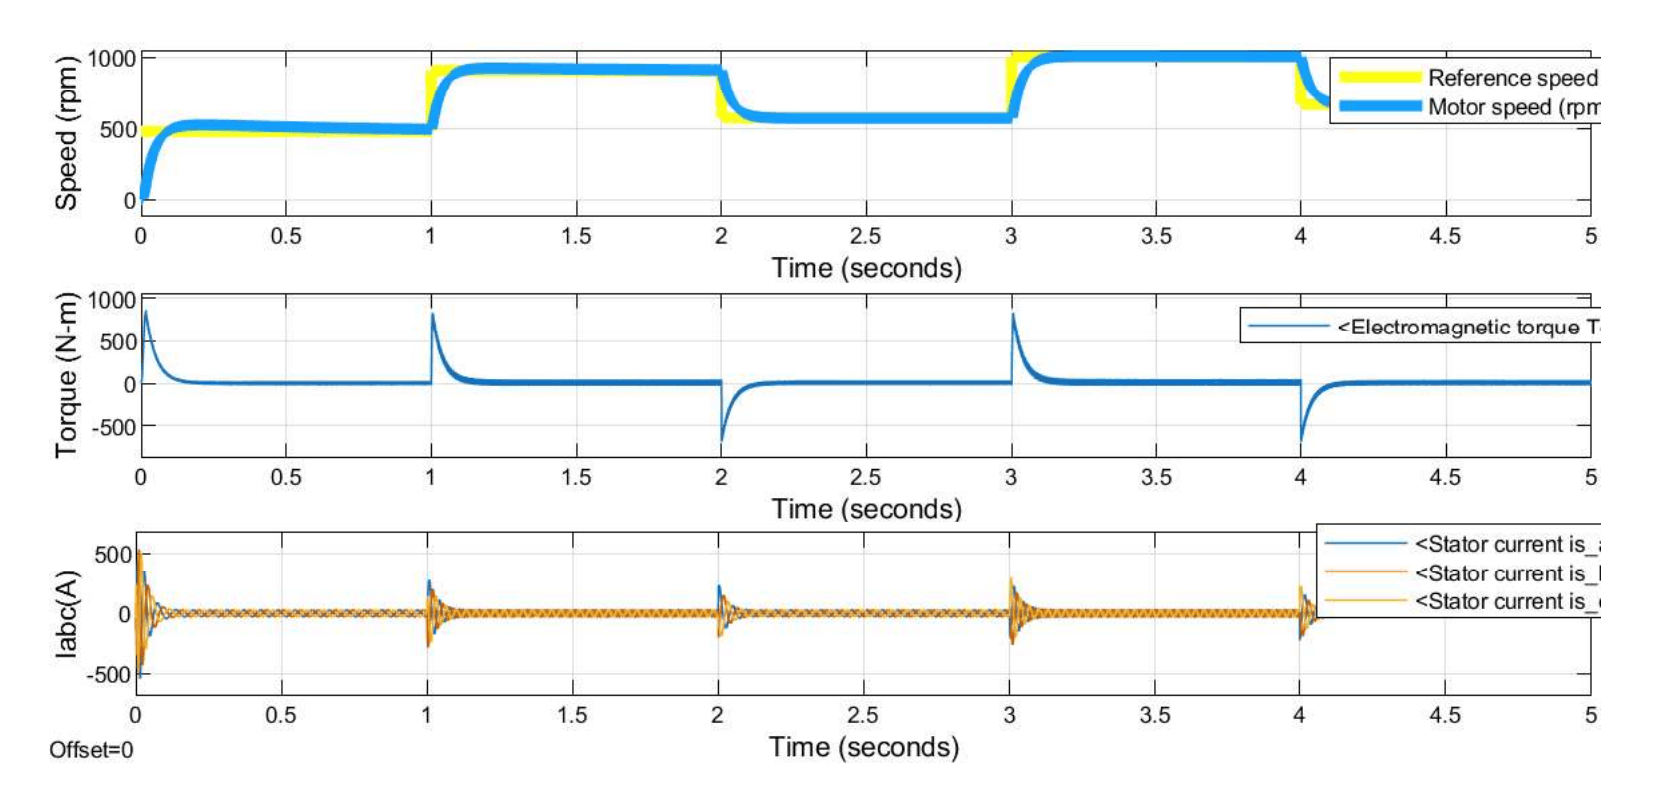
\includegraphics[width=0.9\textwidth]{7.png}
    \caption{Scope Output: Overall Mechanical Dynamics (Speed Tracking, Torque, and Stator Currents)}
    \label{fig:speed_tracking}
\end{figure}

% --- Chapter 3 ---
\chapter{Control System Architecture and Discrete-Time Execution}
The Simulink model is architected around a series of highly deterministic, cascading subsystems executing the Indirect Field Oriented Control (IFOC) algorithm. A critical parameter governing this digital control system is the fundamental sample time, set to $T_s = 2 \mu\text{s}$. This exceptionally fast execution rate ensures stability in the high-bandwidth inner current loops.

\section{Coordinate Transformations}
The central premise of FOC lies in transforming the time-varying, three-phase AC stator variables into a synchronously rotating $d-q$ reference frame.

\subsection{Forward Clarke Transform (Stationary $3\rightarrow2$ Projection)}
The three-phase AC system is projected onto an equivalent two-dimensional orthogonal reference frame ($\alpha-\beta$ axes) using the amplitude-invariant Clarke matrix:
\begin{equation}
\begin{bmatrix} i_{\alpha} \\ i_{\beta} \end{bmatrix} = \frac{2}{3} \begin{bmatrix} 1 & -\frac{1}{2} & -\frac{1}{2} \\ 0 & \frac{\sqrt{3}}{2} & -\frac{\sqrt{3}}{2} \end{bmatrix} \begin{bmatrix} i_{a} \\ i_{b} \\ i_{c} \end{bmatrix}
\end{equation}

\begin{figure}[H]
    \centering
    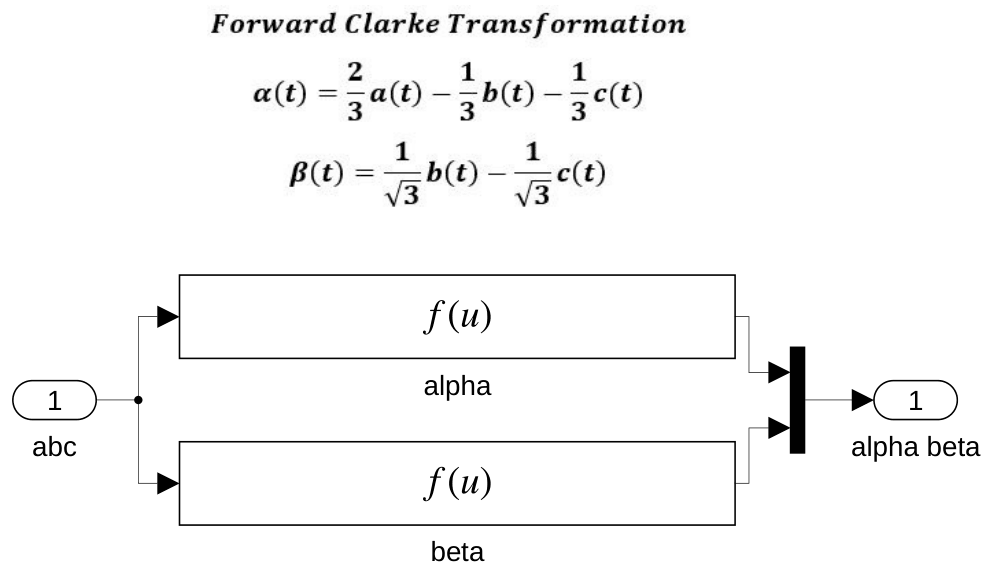
\includegraphics[width=0.7\textwidth]{VECTOR_CONTROL_FOC_OF_IM-06.png}
    \caption{Simulink Subsystem: Forward Clarke Transform ($abc$ to $\alpha\beta$)}
\end{figure}

\subsection{Forward Park Transform (Stationary $\alpha-\beta$ to Rotating $d-q$)}
To allow PI controllers to track signals without steady-state error, the stationary $\alpha-\beta$ frame is projected onto a synchronously rotating reference frame ($d-q$ axes) spinning at the electrical angular velocity of the rotor magnetic flux:
\begin{equation}
\begin{bmatrix} i_{d} \\ i_{q} \end{bmatrix} = \begin{bmatrix} \cos\theta_{e} & \sin\theta_{e} \\ -\sin\theta_{e} & \cos\theta_{e} \end{bmatrix} \begin{bmatrix} i_{\alpha} \\ i_{\beta} \end{bmatrix}
\end{equation}

\begin{figure}[H]
    \centering
    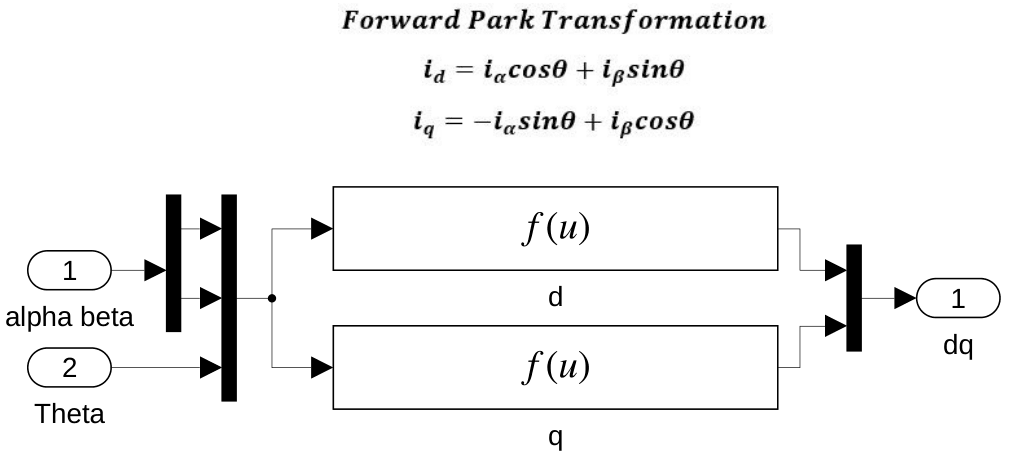
\includegraphics[width=0.7\textwidth]{VECTOR_CONTROL_FOC_OF_IM-07.png}
    \caption{Simulink Subsystem: Forward Park Transform ($\alpha\beta$ to $dq$)}
\end{figure}

\subsection{Reverse Park Transform}
The PI current regulators output decoupling voltage commands ($v_d^*$ and $v_q^*$). The Reverse Park transform performs the coordinate de-rotation back to the stationary frame for the SVPWM block:
\begin{equation}
\begin{bmatrix} v_{\alpha}^* \\ v_{\beta}^* \end{bmatrix} = \begin{bmatrix} \cos\theta_{e} & -\sin\theta_{e} \\ \sin\theta_{e} & \cos\theta_{e} \end{bmatrix} \begin{bmatrix} v_{d}^* \\ v_{q}^* \end{bmatrix}
\end{equation}

\begin{figure}[H]
    \centering
    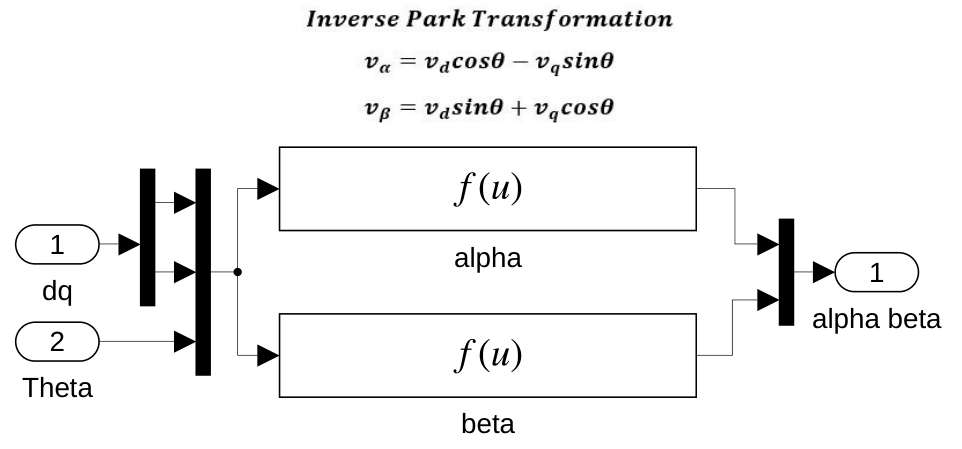
\includegraphics[width=0.7\textwidth]{VECTOR_CONTROL_FOC_OF_IM-09.png}
    \caption{Simulink Subsystem: Reverse Park Transform ($dq$ to $\alpha\beta$)}
\end{figure}

\section{Flux and Torque Decoupling Equations}
\subsection{Direct-Axis Current Reference ($i_{ds}^*$)}
The transient behaviour of the rotor flux linkage $\psi_{r}$ is governed by:
\begin{equation}
\tau_{r}\frac{d\psi_{r}}{dt} + \psi_{r} = L_{m}i_{ds}
\end{equation}
Under the steady-state assumption ($\frac{d\psi_{r}}{dt} = 0$), the reference direct-axis current simplifies to:
\begin{equation}
i_{ds}^* = \frac{\psi_{r}^*}{L_{m}} = \frac{0.96}{0.0347} = 27.6657 \text{ A}
\end{equation}
The d-axis current controller constantly regulates to 27.67 A to maintain nominal flux.

\begin{figure}[H]
    \centering
    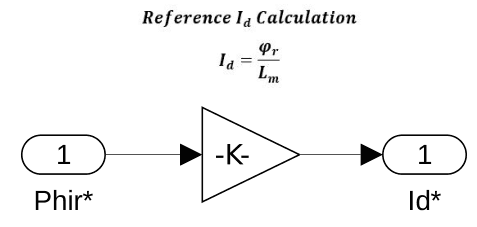
\includegraphics[width=0.6\textwidth]{VECTOR_CONTROL_FOC_OF_IM-03.png}
    \caption{Simulink Subsystem: $I_d^*$ Reference Calculation}
\end{figure}

\subsection{Quadrature-Axis Current Reference ($i_{qs}^*$)}
Aligning the d-axis perfectly with the rotor flux vector forces $\psi_{qr} = 0$. The torque equation becomes:
\begin{equation}
T_{e} = \frac{3}{2}\left(\frac{P}{2}\right)\frac{L_{m}}{L_{r}}\psi_{r}i_{qs}
\end{equation}
Inverting this to solve for the necessary reference current $i_{qs}^*$:
\begin{align}
i_{qs}^* &= \frac{2}{3} \cdot \frac{2}{P} \cdot \frac{L_{lr} + L_{m}}{L_{m}} \cdot \frac{T_{e}^*}{\psi_{r}} \\
i_{qs}^* &= \left(\frac{2}{3}\right) \left(\frac{2}{4}\right) \left(\frac{0.0355}{0.0347}\right) \frac{T_{e}^*}{0.96} \\
i_{qs}^* &= (0.3333) \times (1.02305) \times \frac{T_{e}^*}{0.96} = 0.3552 \cdot T_{e}^* \text{ A}
\end{align}

To prevent a division-by-zero singularity during startup when $\psi_r \approx 0$, the digital implementation adds a numerical perturbation ($\epsilon = 1 \times 10^{-3}$):
\begin{equation}
i_{qs}^* \propto \frac{T_{e}^*}{\psi_{r} + 10^{-3}}
\end{equation}

\begin{figure}[H]
    \centering
    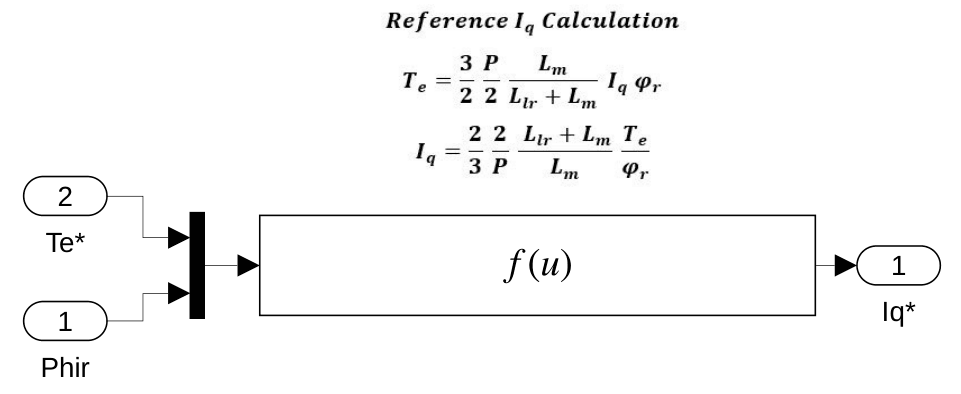
\includegraphics[width=0.8\textwidth]{VECTOR_CONTROL_FOC_OF_IM-04.png}
    \caption{Simulink Subsystem: $I_q^*$ Reference Calculation}
\end{figure}

\section{Slip and Flux Angle ($\theta_e$) Synthesis}
Indirect FOC synthesises the flux angle mathematically in a feedforward manner by calculating the required slip frequency ($\omega_{sl}$):
\begin{equation}
\omega_{sl} = \frac{L_{m}}{\tau_{r}} \cdot \frac{i_{qs}^*}{\psi_{r}^*} = \frac{0.0347}{0.1557} \cdot \frac{i_{qs}^*}{0.96} = 0.232 \cdot i_{qs}^* \text{ rad/s}
\end{equation}

The synchronous speed ($\omega_e$) is found by adding the slip to the electrical rotor speed ($\omega_r = \omega_m \frac{P}{2}$):
\begin{equation}
\omega_{e} = \omega_{r} + \omega_{sl} = 2\omega_{m} + 0.232 \cdot i_{qs}^* \text{ rad/s}
\end{equation}

The instantaneous rotor flux angle is obtained via discrete integration ($T_s = 2 \mu\text{s}$):
\begin{equation}
\theta_{e}[k] = (\theta_{e}[k-1] + \omega_{e}[k] \cdot T_{s}) \pmod{2\pi}
\end{equation}

\begin{figure}[H]
    \centering
    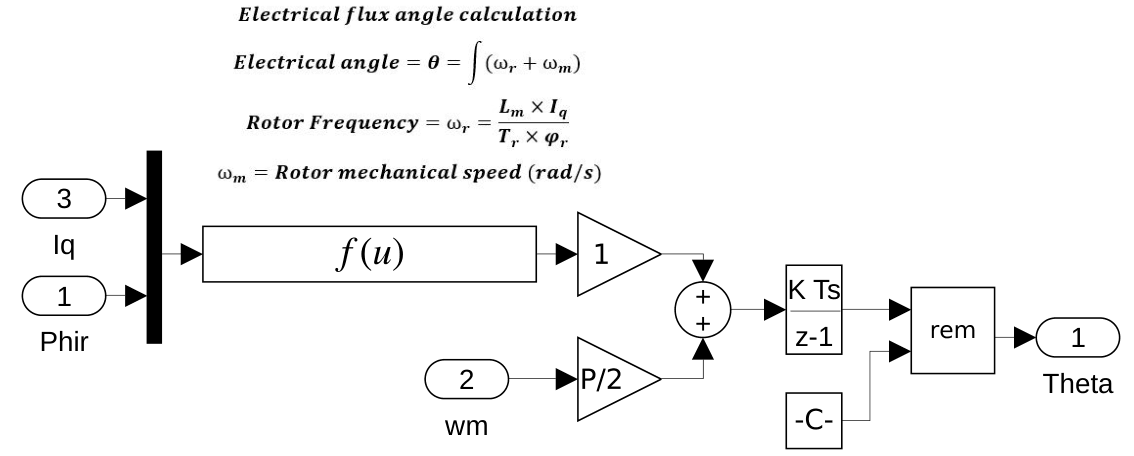
\includegraphics[width=0.8\textwidth]{VECTOR_CONTROL_FOC_OF_IM-05.png}
    \caption{Simulink Subsystem: IFOC Slip and Flux Angle Estimation}
\end{figure}

\begin{figure}[H]
    \centering
    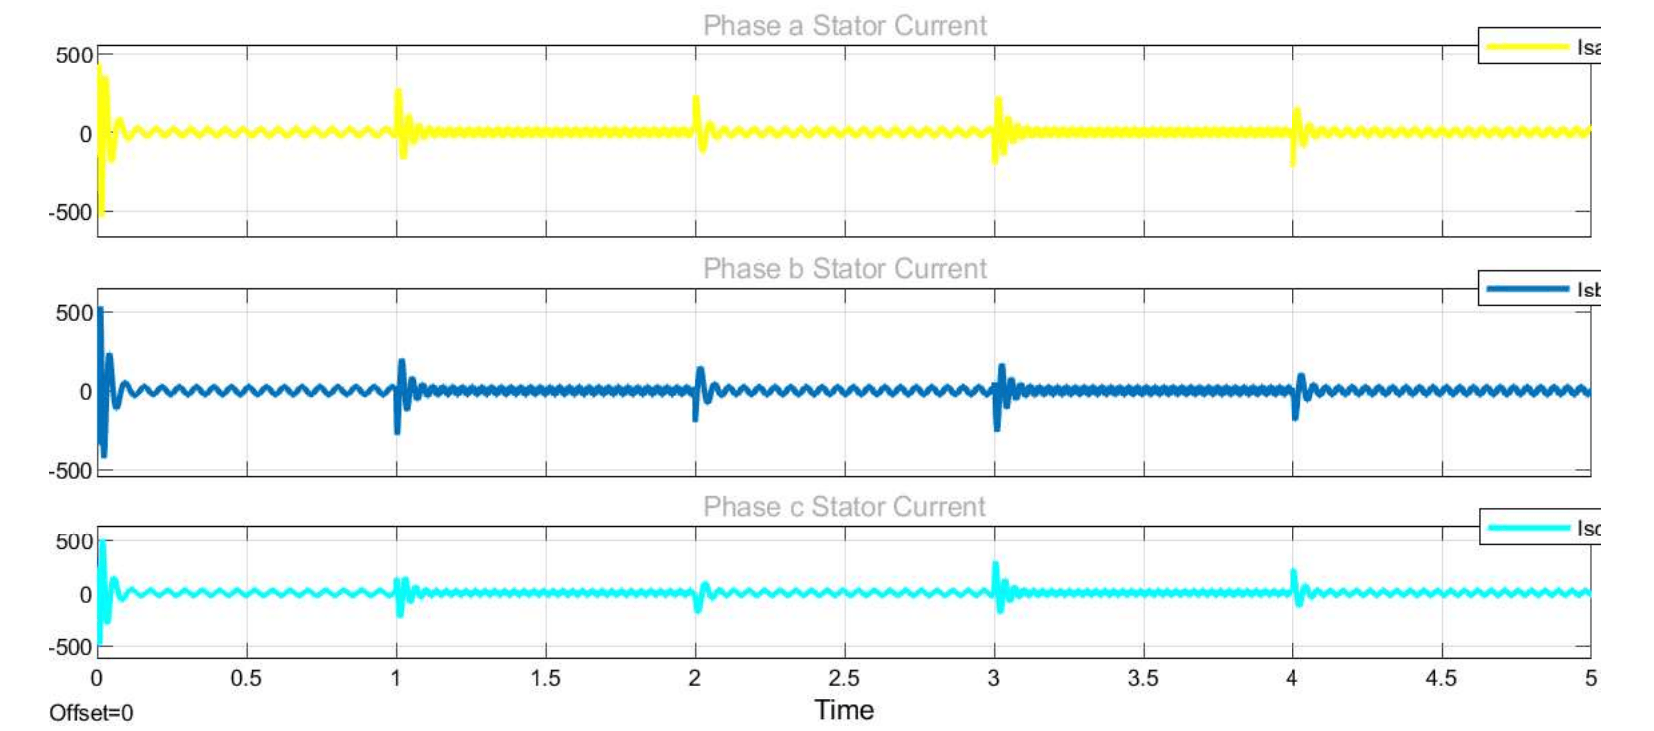
\includegraphics[width=0.9\textwidth]{23.png}
    \caption{Scope Output: Three-Phase Stator Currents ($I_a$, $I_b$, $I_c$) Responding to Load Transients}
\end{figure}


% --- Chapter 4 ---
\chapter{Space Vector Pulse Width Modulation (SVPWM)}
The final control actuation is executed by a Three-Phase Voltage Source Inverter, powered by a 780 V DC link. The Space Vector PWM (SVPWM) subsystem translates continuous domain $v_\alpha^*$ and $v_\beta^*$ voltage commands into discrete transistor switching signals, optimising DC bus utilisation by up to 15.47\% over standard SPWM and significantly reducing total harmonic distortion.

\begin{figure}[H]
    \centering
    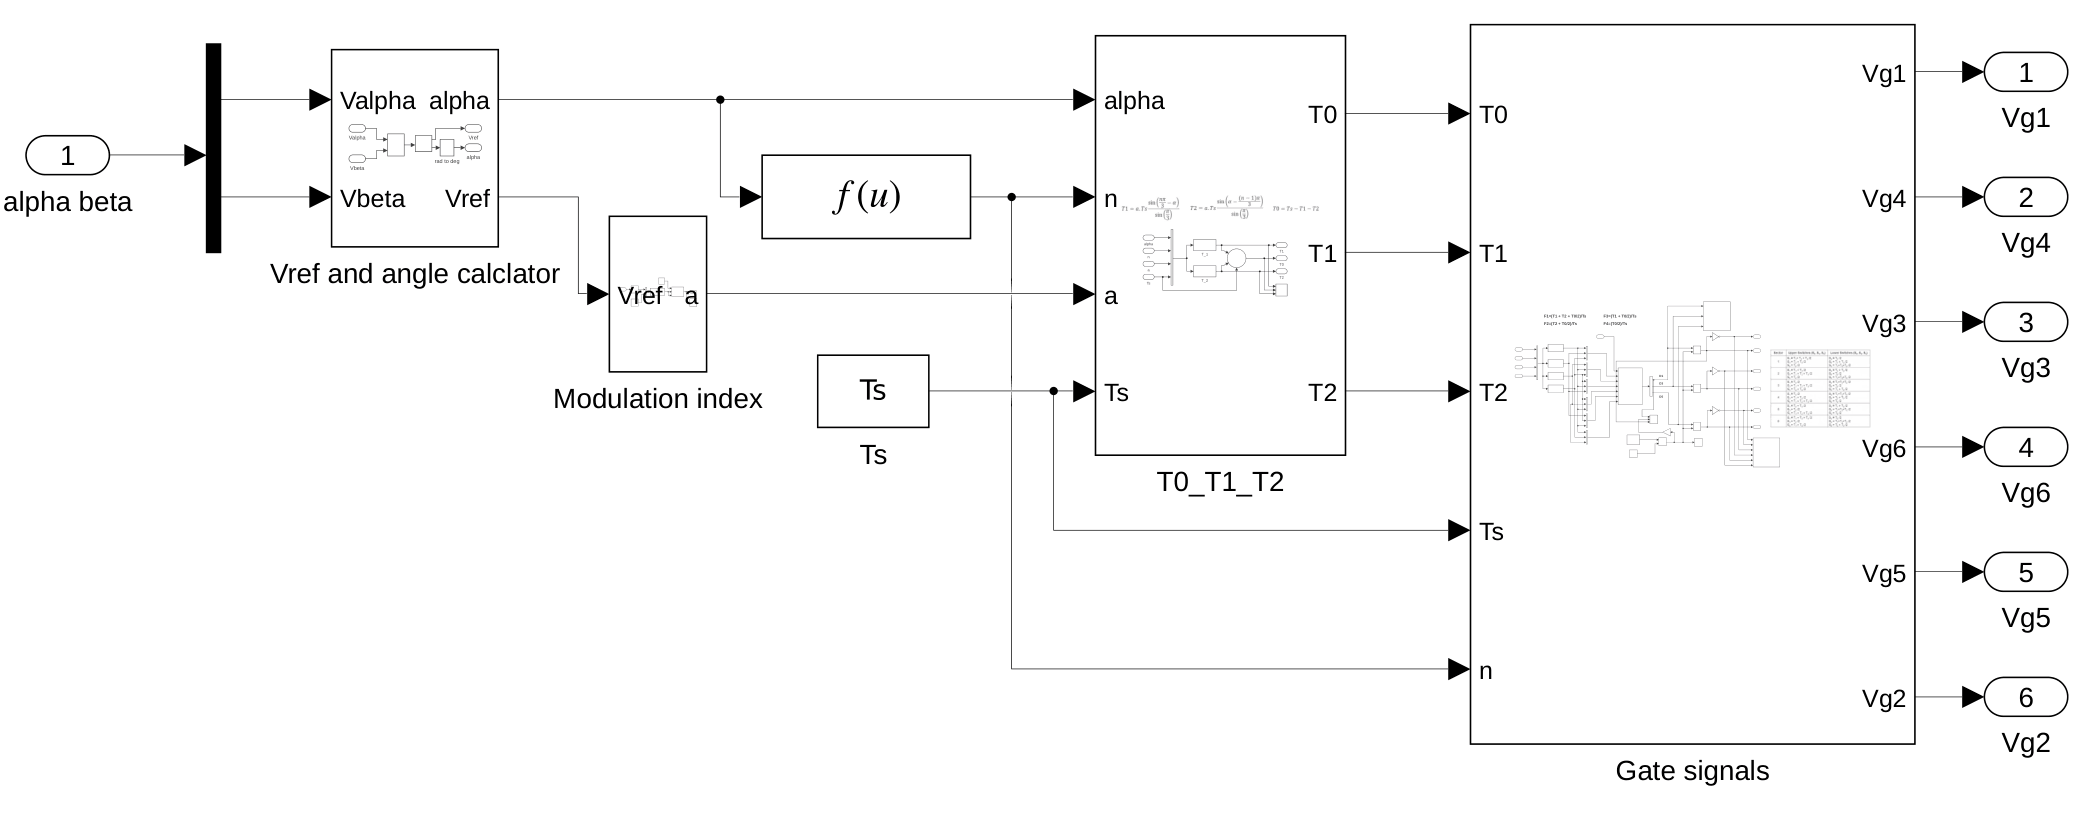
\includegraphics[width=0.9\textwidth]{VECTOR_CONTROL_FOC_OF_IM-10.png}
    \caption{Main Architecture of the Space Vector PWM Generation Subsystem}
\end{figure}

\section{SVPWM Algorithm Execution}
\subsection{Reference Vector Synthesis and Modulation Index}
The model computes the magnitude and angle of the reference vector:
\begin{equation}
|\vec{V}_{ref}| = \sqrt{(v_{\alpha}^*)^2 + (v_{\beta}^*)^2}
\end{equation}
\begin{equation}
\theta_{ref} = \arctan\left(\frac{v_{\beta}^*}{v_{\alpha}^*}\right)
\end{equation}

\begin{figure}[H]
    \centering
    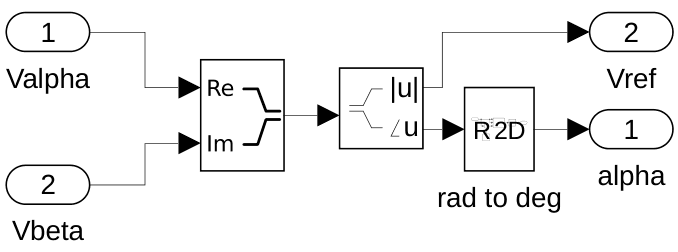
\includegraphics[width=0.6\textwidth]{VECTOR_CONTROL_FOC_OF_IM-14.png}
    \caption{Simulink Subsystem: Transformation to Magnitude ($V_{ref}$) and Angle ($\alpha$)}
\end{figure}

To prevent non-linear operation, the modulation index $a$ is bounded:
\begin{equation}
a = \frac{\sqrt{3} \cdot |\vec{V}_{ref}|}{V_{dc}} \le 0.866
\end{equation}

\begin{figure}[H]
    \centering
    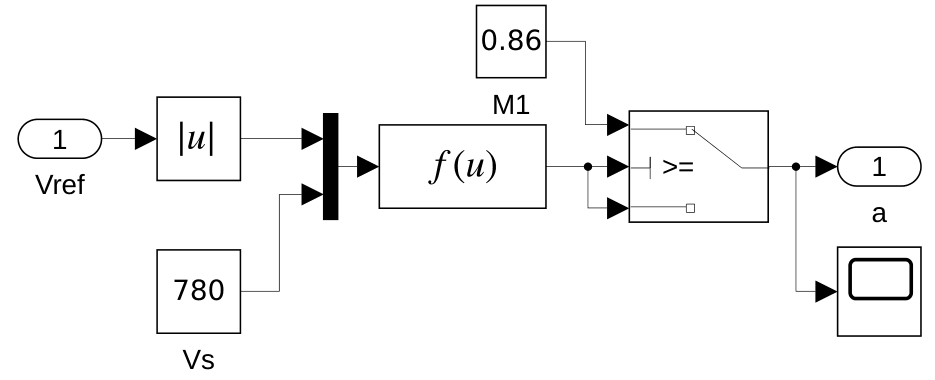
\includegraphics[width=0.6\textwidth]{VECTOR_CONTROL_FOC_OF_IM-12.png}
    \caption{Simulink Subsystem: Modulation Index Calculation}
\end{figure}

\subsection{Dwell Time Calculation}
The dwell times for the active vectors are calculated using the volt-second balance principle over switching period $T_s$:
\begin{align}
T_{1} &= a \cdot T_{s} \cdot \frac{\sin\left(\frac{n\pi}{3} - \alpha\right)}{\sin\left(\frac{\pi}{3}\right)} \\
T_{2} &= a \cdot T_{s} \cdot \frac{\sin\left(\alpha - \frac{(n-1)\pi}{3}\right)}{\sin\left(\frac{\pi}{3}\right)} \\
T_{0} &= T_{s} - T_{1} - T_{2}
\end{align}

\begin{figure}[H]
    \centering
    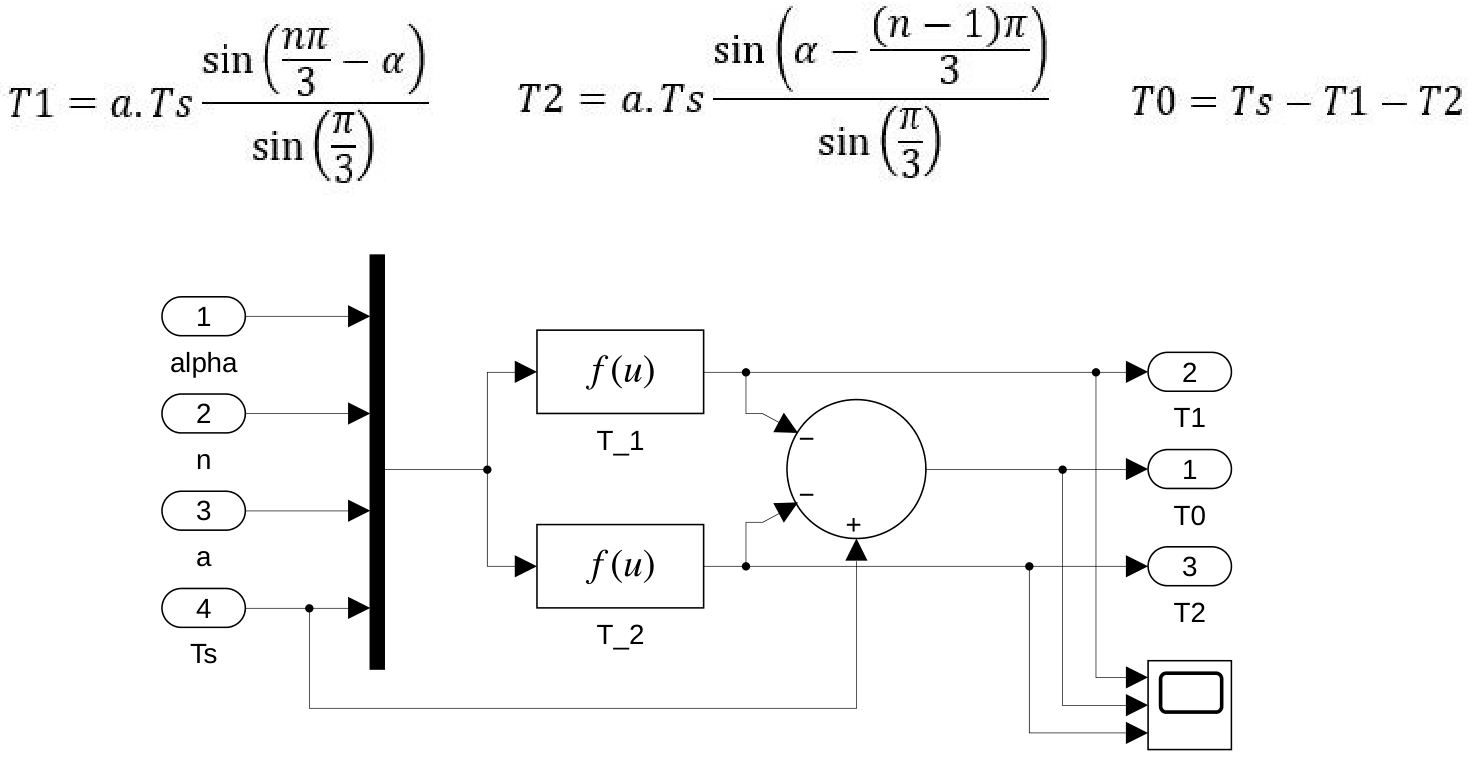
\includegraphics[width=0.8\textwidth]{VECTOR_CONTROL_FOC_OF_IM-13.png}
    \caption{Simulink Subsystem: Dwell Time ($T_1, T_2, T_0$) Calculation}
\end{figure}

\begin{figure}[H]
    \centering
    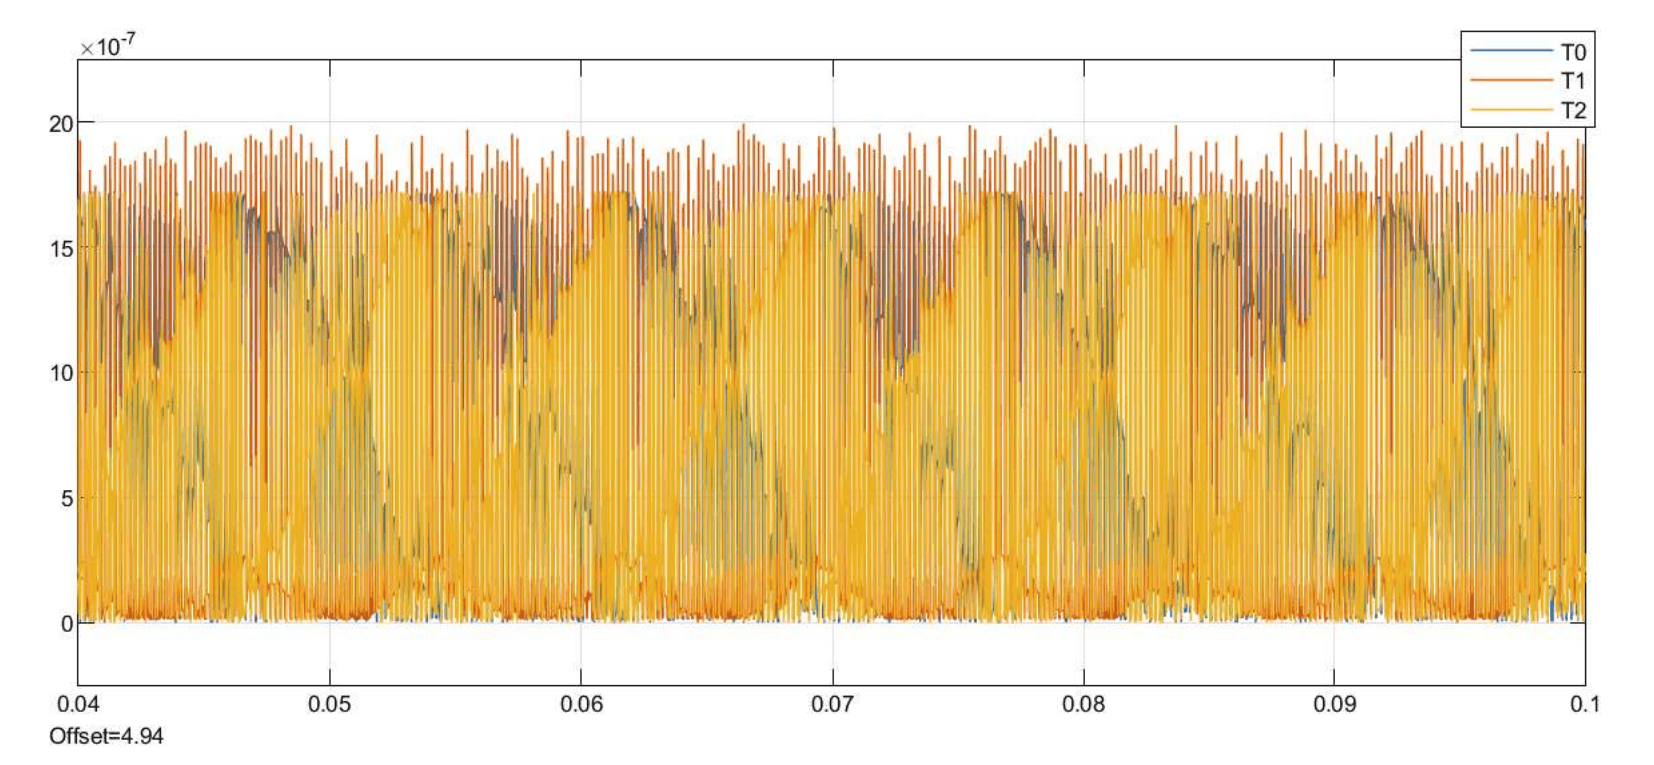
\includegraphics[width=0.9\textwidth]{31.png}
    \caption{Scope Output: Calculated High-Frequency Dwell Times}
\end{figure}

\subsection{Switching Sequence Generation}
The calculated dwell times are mapped to logical duty cycle values via a multiport switch governed by the sector number $n$, which are then compared against a high-frequency triangular carrier to generate physical Boolean pulses ($V_{g1}$ to $V_{g6}$) for the IGBT drivers. A symmetrical switching pattern ($\vec{V}_{0} \rightarrow \vec{V}_{1} \rightarrow \vec{V}_{2} \rightarrow \vec{V}_{7} \rightarrow \vec{V}_{2} \rightarrow \vec{V}_{1} \rightarrow \vec{V}_{0}$) is employed.

\begin{figure}[H]
    \centering
    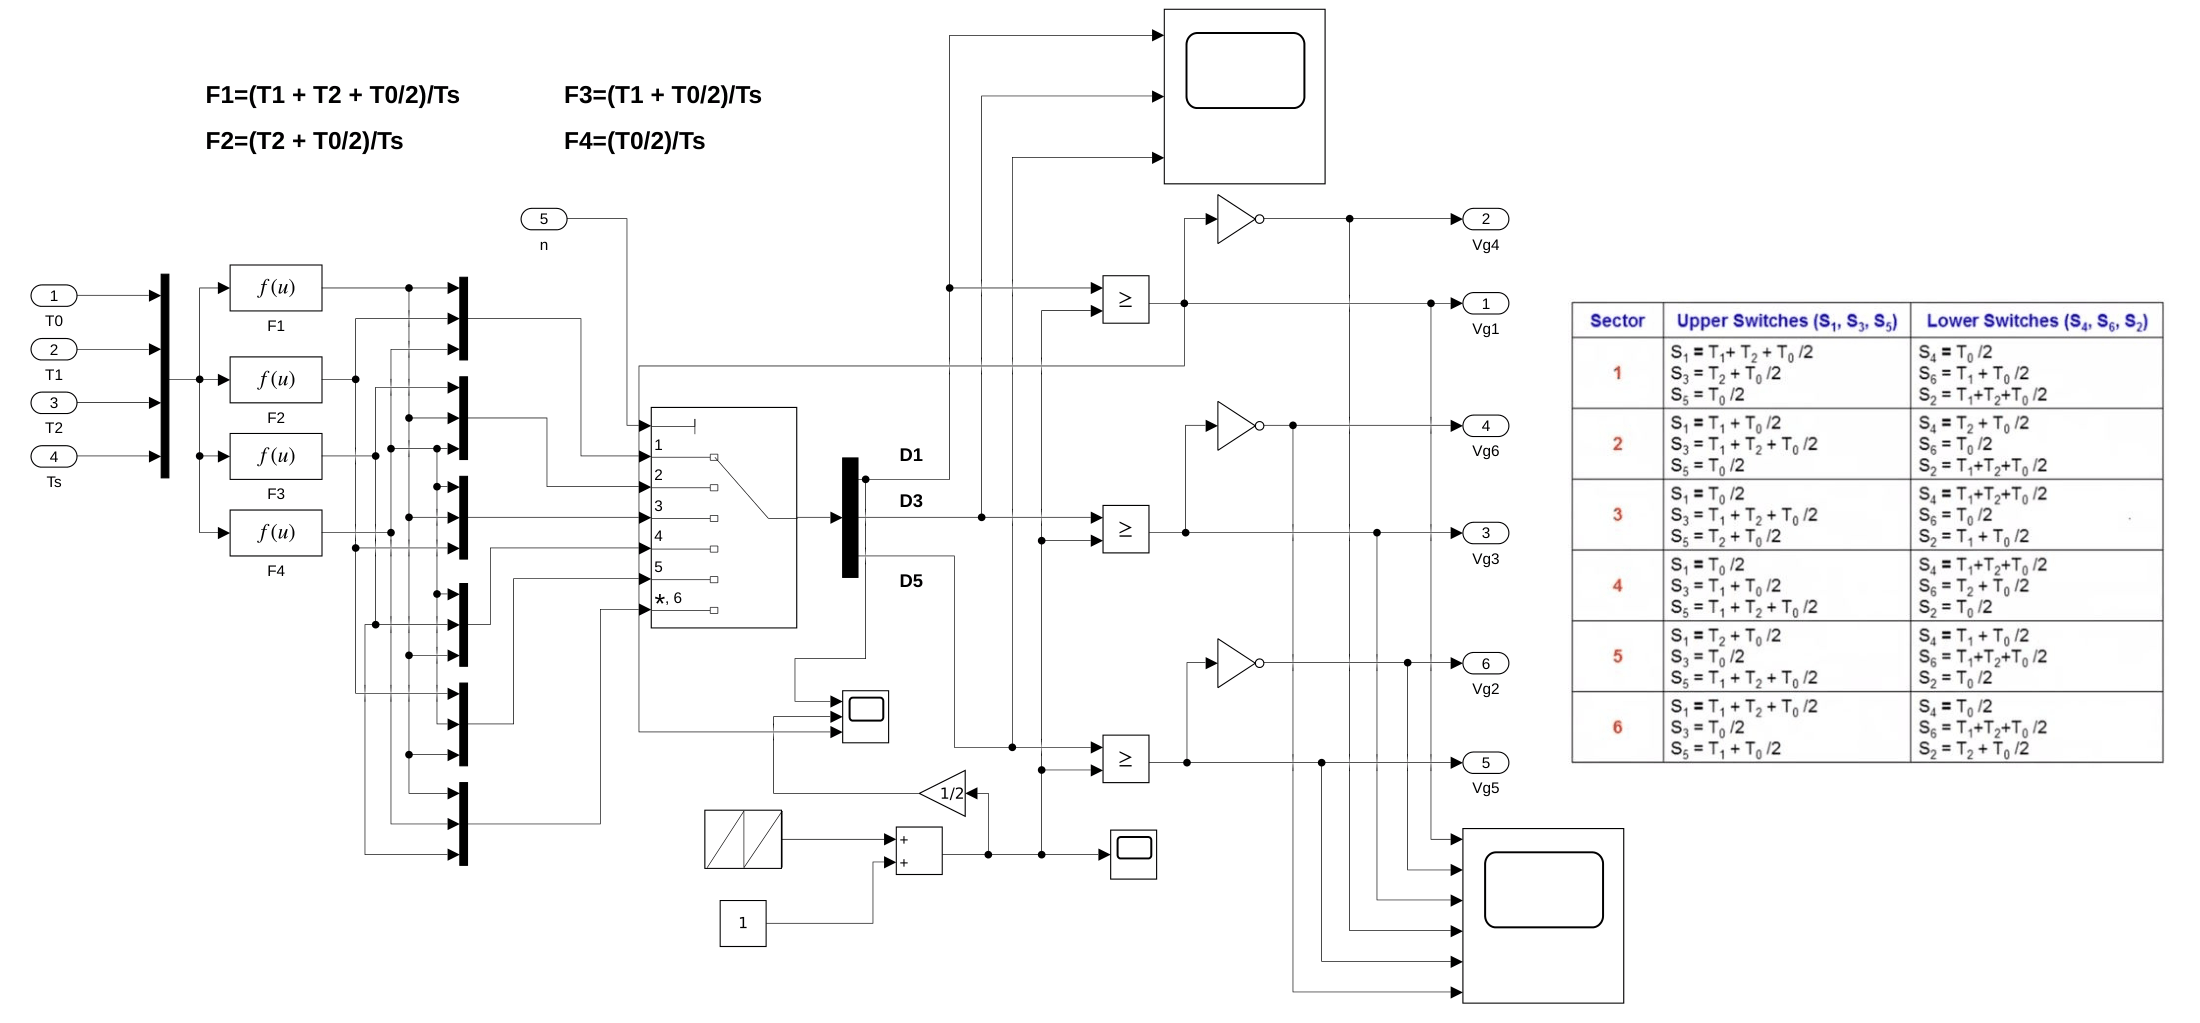
\includegraphics[width=0.9\textwidth]{VECTOR_CONTROL_FOC_OF_IM-11.png}
    \caption{Simulink Subsystem: Detailed PWM Logic and Gate Signal Comparator Routing}
\end{figure}

\begin{figure}[H]
    \centering
    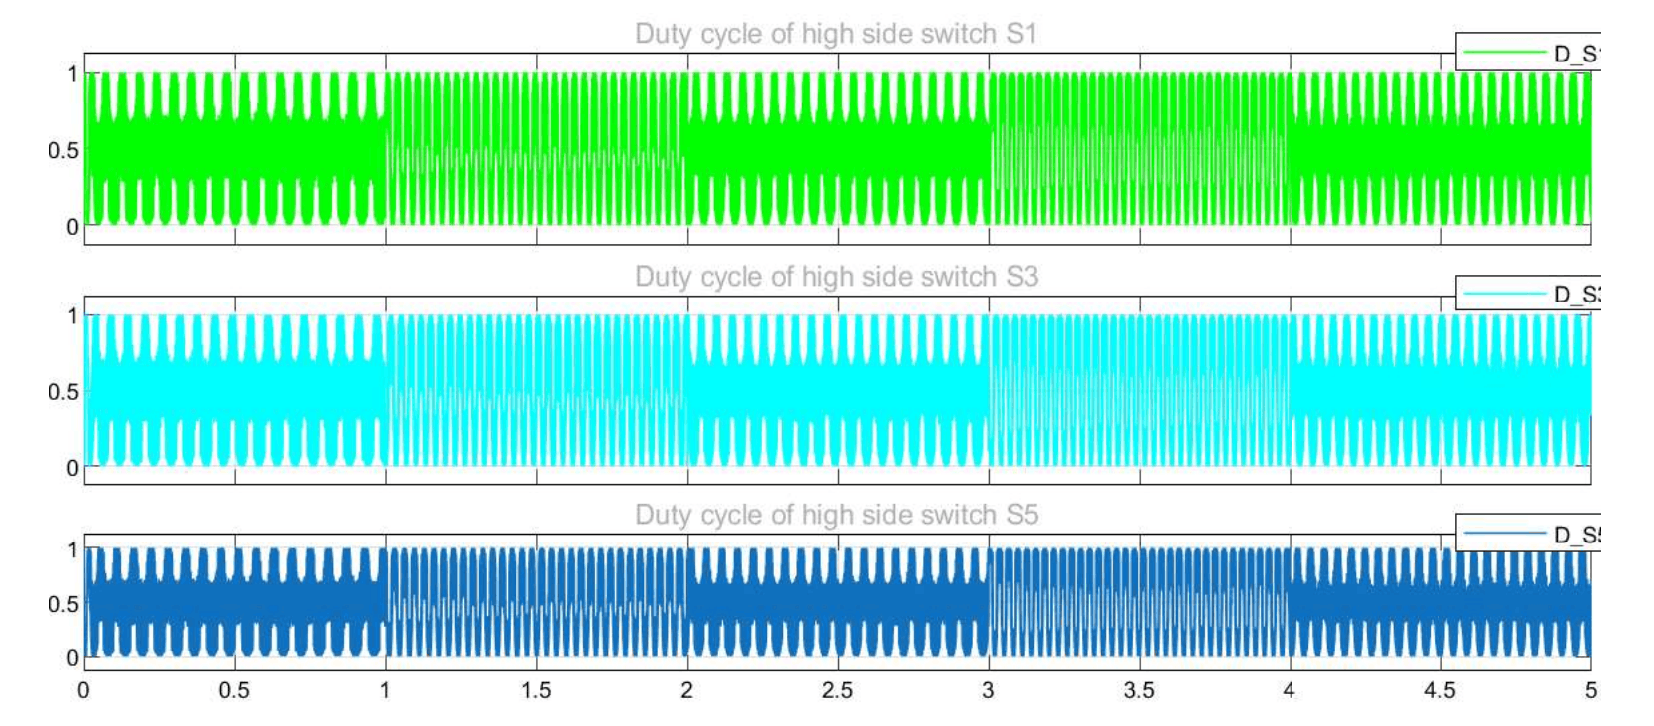
\includegraphics[width=0.9\textwidth]{32.png}
    \caption{Scope Output: Duty Cycles of the High-Side Inverter Switches}
\end{figure}

\begin{figure}[H]
    \centering
    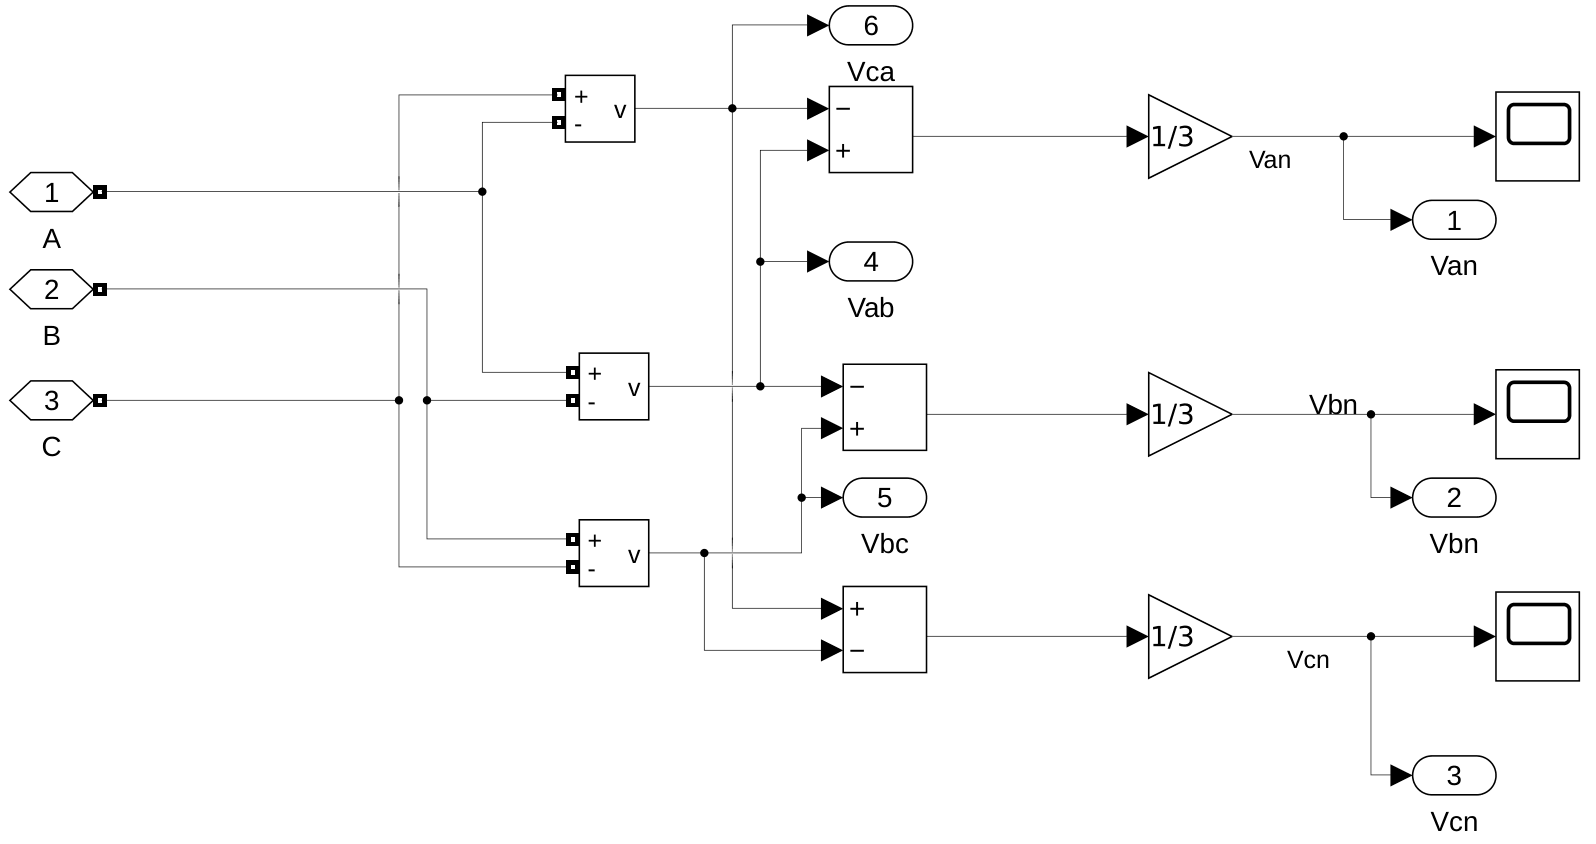
\includegraphics[width=0.8\textwidth]{VECTOR_CONTROL_FOC_OF_IM-08.png}
    \caption{Simulink Subsystem: Three-Phase and Line-to-Line Inverter Voltage Calculation}
\end{figure}

% --- Chapter 5 ---
\chapter{Conclusion and Future Scope}
\section{Conclusion}
The presented Simulink model serves as a highly accurate, functionally complete digital twin of a modern, industrial-grade Indirect Field Oriented Control (IFOC) system for a Squirrel-Cage Induction Motor. By meticulously modelling the electromechanical plant, the coordinate transformations, and the discrete-time control logic, this architecture successfully demystifies the complex, non-linear dynamics inherent in three-phase AC machines.

The mathematical projection of the stator currents into a synchronously rotating $d-q$ reference frame proves that an induction motor can be controlled with the same orthogonal precision, and dynamic transient response, as a separately excited DC motor. Operating at a stringent $2 \mu\text{s}$ sample time, the model faithfully replicates the execution environment of a modern Digital Signal Processor (DSP), highlighting the necessary bandwidth separation between the slower, inertia-dominated outer speed loop and the high-bandwidth inner PI current regulators. The integration of Space Vector PWM further verifies the capability to maximise DC bus utilisation and suppress harmonic distortion, making this a complete and robust control strategy.

\section{Future Scope}
Future enhancements to this control architecture could include:
\begin{itemize}
    \item \textbf{Sensorless Control Integration:} Replacing the mechanical speed sensor with a Model Reference Adaptive System (MRAS) or Extended Kalman Filter (EKF) to estimate rotor speed purely from terminal voltages and currents.
    \item \textbf{Online Parameter Identification:} Implementing an adaptive algorithm to estimate the rotor resistance ($R_r$) in real-time, preventing IFOC detuning due to thermal variations during extended operation.
    \item \textbf{Field Weakening Operation:} Extending the control algorithm to dynamically attenuate $i_{ds}$ when operating above base speed, allowing the motor to enter the constant-power region.
\end{itemize}

\end{document}
